\begin{document}

Cluster analysis is \guillemotleft the task of grouping a set of objects in such a way that objects in the same group are more similar to each other than to those in other groups. It is a main task of exploratory data mining, and a common technique for statistical data analysis, used in many fields \guillemotright \footnote{Clustering: \url{http://shodhganga.inflibnet.ac.in/bitstream/10603/36013/11/chapter7.pdf}}.

\subsection{Data used}

Our original dataset had 8387 records, where each one had 190 variables. More than 100 variables are numerical (some repeated or for different waves), 6 variables are binary and 19 variables are qualitative. The dataset has a 26.44\% of missing data.

After pre-processing our dataset has 3656 rows, where each one had 36 variables. 20 variables are numerical, 6 variables are categorical and 5 variables are binary.

\subsection{Clustering method used}
As requested in the instructions for this project, we will perform a hierarchical clustering.

To solve the problem of having numerical and categorical variables at the same time we will be using the Gower distance, which generates an $N^2$ {end} distance matrix.

After that, for the hierarchical clustering analysis of our dataset, we have used Ward's minimum variance method, which is based on the general agglomerative hierarchical clustering procedure. Basically, this method can be understood as follows. We choose the two groups to merge by looking at the value of an objective function which we want to optimize. In the case of Ward's minimum variance method, the objective function is the error sum of squares. This method takes into account the variance instead of using distance metrics and it generates a tree. We will cut the tree in such a way that we obtain the desired number of clusters. We will use R packages that implement this method \footnote{Agglomerative Hierarchical Clustering: \url{https://onlinecourses.science.psu.edu/stat505/node/143/}}.



\newpage
\subsection{Discuss about number of clusters}

There are many different methods in order to determine what is the optimal number of segment. The decision might be subjective and it depends on the method used. One of them relays on visual assessment by visually inspect the dendogram in order to decide if the tree suggest a particular number of clusters, but this method is also subjective \footnote{Determining the optimal number of clusters: 3 must known methods - Unsupervised Machine Learning}{\url{http://www.sthda.com/english/wiki/print.php?id=239}}.

Nevertheless, there is another method using some existing algorithms that somehow can help help us to take the right choice in a more objective way.

These algorithms include using a R function from \emph{factoextra}
package: \emph{fviz\_nbclust()}.
We used two different methods, which are: elbow method and silhouette.

We can see from the two figures below the optimal clusters number according to these algorithms: 3.

\begin{figure}[ht]
  \centering
  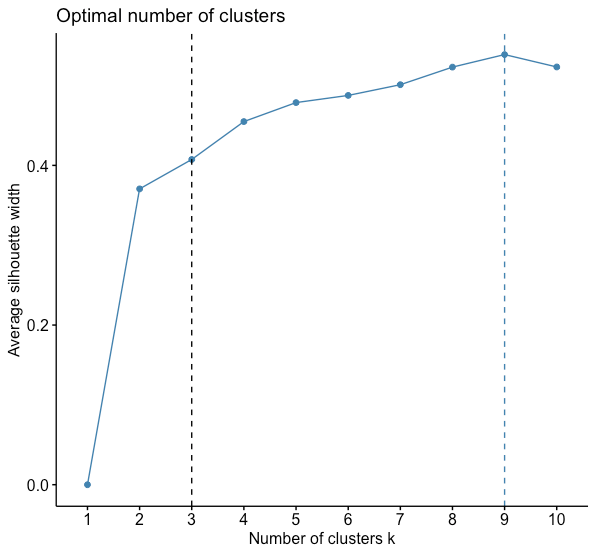
\includegraphics[width= 7cm]{images/ClusterPlot2.png}
  \caption{Optimal number of clusters using Silhouette method.}
  \label{fig:indiv}
\end{figure}

\begin{figure}
  \centering
  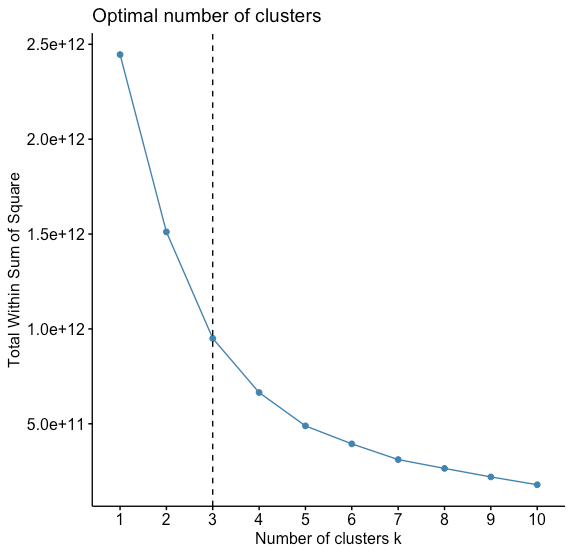
\includegraphics[width= 7cm]{images/ClusterPlot1.png}
  \caption{Optimal number of clusters using Elbow method.}
  \label{fig:indiv}
\end{figure}


\newpage
\subsection{Clusters size}

We can see in the table below the amount of data in each cluster.

\begin{table}[h!]
\centering
\begin{tabular}{|c| c|} 
 \hline
 \textbf{Cluster} & \textbf{Number of rows} \\ [0.5ex]
 \hline\hline
 1 & 1600\\
 2 & 1213\\
 3 & 843\\
 \hline
\end{tabular}
\caption{Size of each cluster}
\label{table:1}
\end{table}

\begin{figure}
  \subsection{Resulting dendogram}
  \centering
  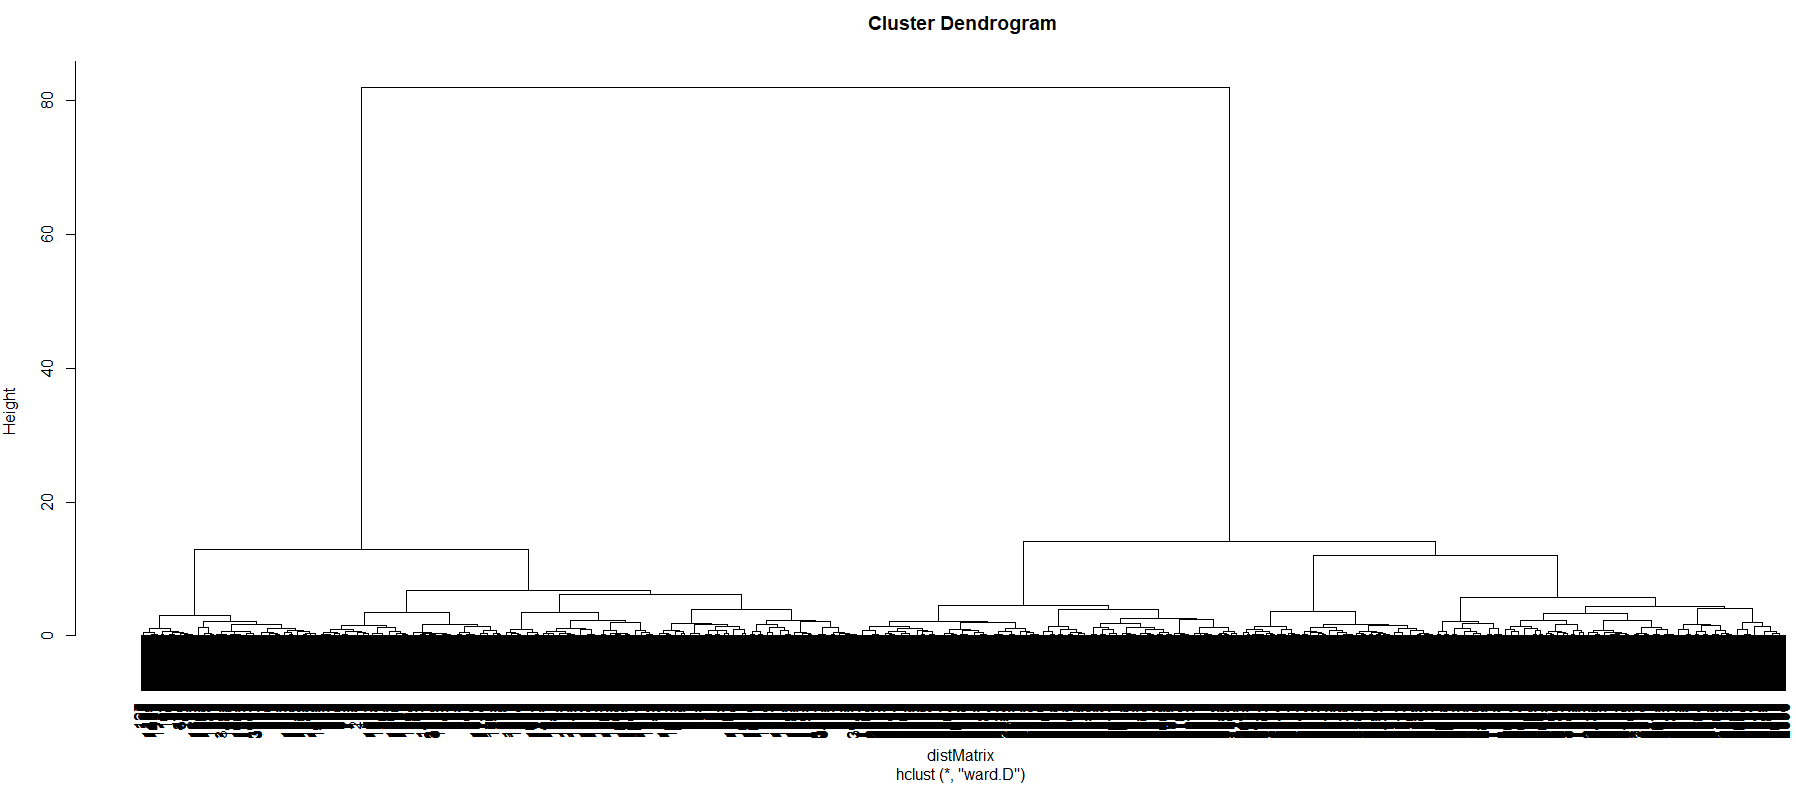
\includegraphics[angle = 90, width= 9cm]{images/endograma.png}
  \caption{Dataset clusters dendogram.}
  \label{fig:indiv}
\end{figure}

\end{document}
